\chapter[Tuning the parameters of the SNN]{Tuning the parameters of the SNN\raisebox{.15\baselineskip}{\Large\footnotemark}}
\footnotetext{The results of this chapter were submitted as \textit{Recapitulating the electrophysiological features of in vivo biological networks by using a real-time hardware Spiking Neural Network} for the EMBC 2024 conference. The analysis conducted here is also included in the article titled \textit{BiœmuS: A New Tool for Studying Neurological Disorders Through Real-Time Emulation and Hybridization Using Biomimetic Spiking Neural Networks}, currently under review for publication in Nature Communications.}

\section{Introduction}

This work aims to advance the development of a device for delivering a novel personalized stimulation for post-stroke rehabilitation. As seen before, a promising therapy involves electrical stimulation to establish new connections between separated brain regions, leveraging neural plasticity. Closed-loop stimulation has shown promise in restoring lost abilities in rats \cite{Guggenmos2013,Averna2020,Averna2021}, unlike traditional open-loop paradigms.

This study proposes a tuning phase of a hardware-based SNN \cite{Beaubois2023} for a new open-loop approach that maintains the bio-mimetic nature of stimulation. The spontaneous activity of the RFA area of six healthy adult anesthetized rats was analyzed to extract key electrophysiological features required for customizing SNN parameters (Figure \ref{fig:Biomimetic Approach}).

Various SNNs were built, and comparative analyses between the electrical patterns generated by SNNs and the neural activity recorded from the BNNs were performed. By identifying the SNN that best matches the pool of electrophysiological features observed in vivo, in the future, it may be possible to stimulate the S1 area with a pattern derived from the activity of the digital twin of a BNN.

\begin{figure}[ht!]
    \begin{center}
    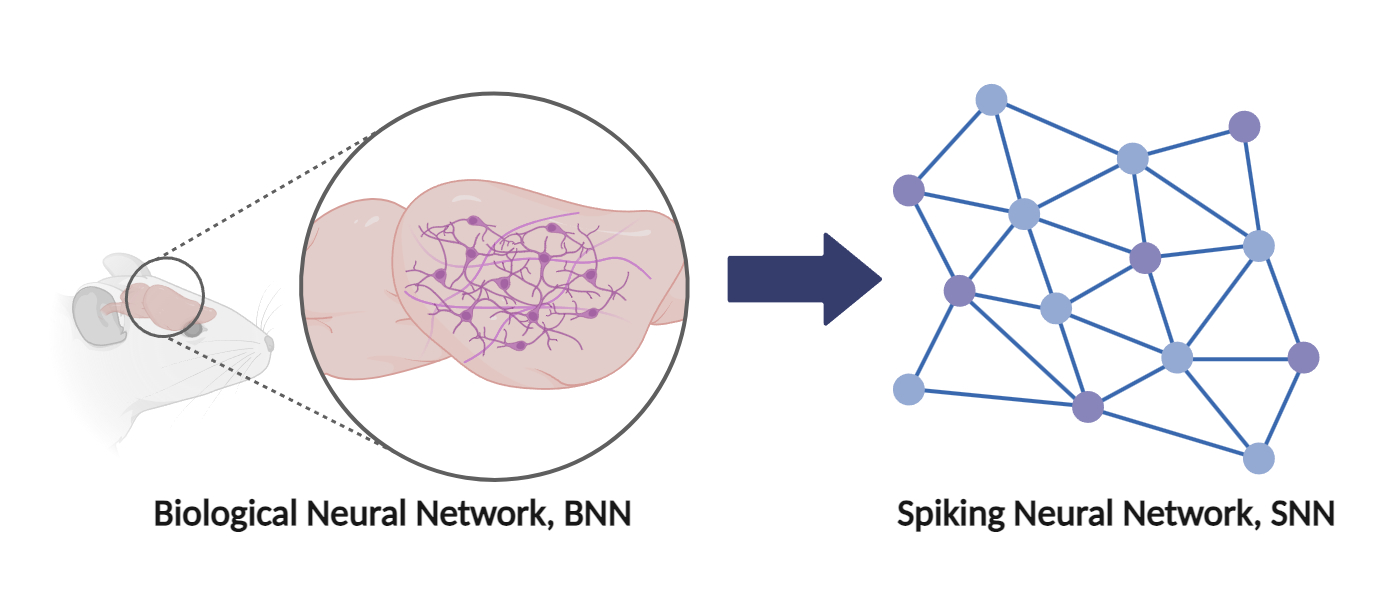
\includegraphics[width=0.9\linewidth]{Figure/Biomimetic Approach.jpg}
    \end{center}
    \caption{Schematic representation of the bio-mimetic approach (from BNN to SNN).}
    \label{fig:Biomimetic Approach}
\end{figure}

\section{Materials and Methods}

\subsection{Biological Neural Network (BNN)}

The biological model that constitutes the Biological Neural Network is derived solely from the RFA area of six animals, chosen based on the shape of their ISIH through visual inspection among those introduced in the previous chapter. Specifically, for the subsequent analyses, only the first 10 minutes of spontaneous activity recorded in the PreL phase of the experimental procedure, outlined in the section "Experimental Protocol" of the previous chapter, are considered to characterize the behavior of a healthy network.

\subsection{Spiking Neural Network (SNN)}

The digital platform employed for the development of the bio-mimetic SNN is a System on Chip (SoC) FPGA based on the Zynq™ UltraScale+ MPSoC architecture (Figure \ref{fig:SoC FPGA}). This platform integrates CPU cores, referred to as software part, and programmable logic (FPGA), referred to as hardware part \cite{Beaubois2023}, on the same chip. 

\begin{figure}[ht!]
    \begin{center}
    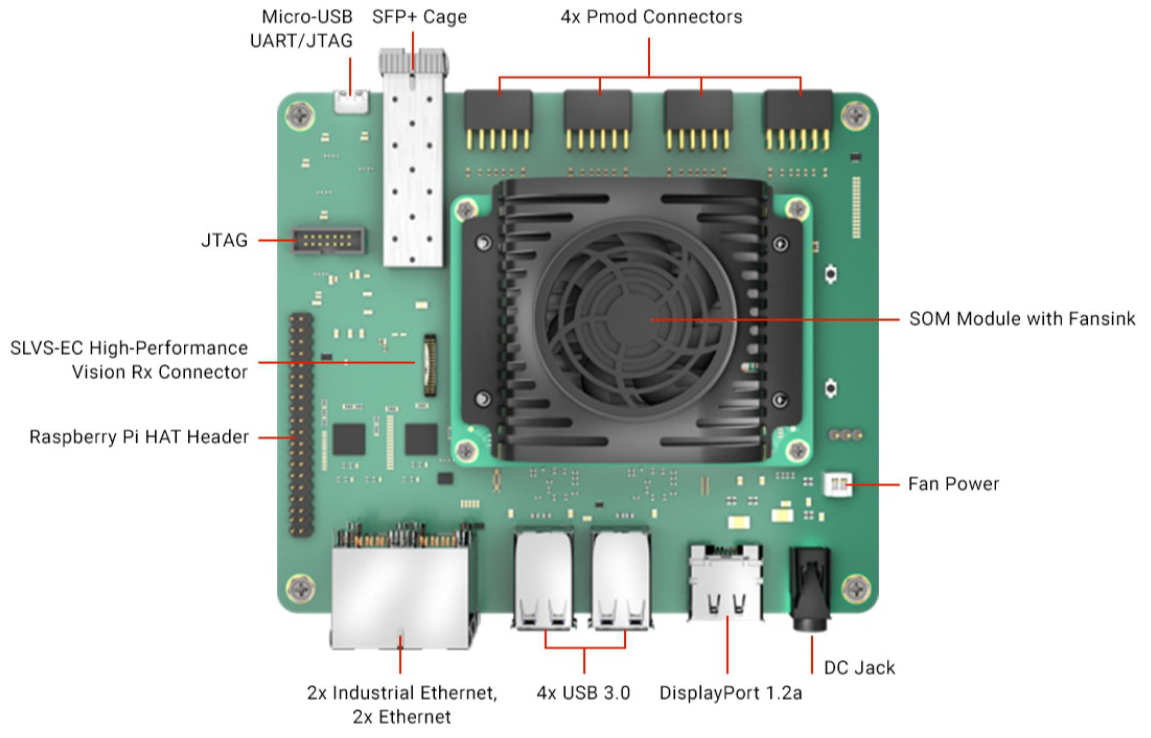
\includegraphics[width=0.9\linewidth]{Figure/SoC FPGA.jpg}
    \end{center}
    \caption{Kria K26 SOM from AMD Xilinx embedded on the development platforms Kria KR260 Robotics Starter Kit. From [https://www.amd.com/en/products/system-on-modules/kria/k26/kr260-robotics-starter-kit.html].}
    \label{fig:SoC FPGA}
\end{figure}

The compact design of the carrier boards, coupled with their flexibility and high processing performance, presents notable advantages for integration into a biohybrid experimental setup.

The system used, capable of running up to 1024 single-compartment neurons fully connected and supporting a total of 2\textsuperscript{20} synapses, is named Bi{\oe}muS, which stands for "\textbf{BIO}mimetic \textbf{EMU}lation \textbf{S}ingle compartment." It incorporates on-board monitoring and provides versatile external communication options, such as Ethernet or WiFi. 

Python scripts enable the configuration and monitoring of the system. They generate two files - one for hardware and one for software configuration of the SoC FPGA (see Figure \ref{fig:Architecture BioEmus}). The software configuration is specified by the file in JSON format (e.g. \textit{swconfig.json}), encompassing various parameters like the path to the hardware configuration file, emulation time, configuration of different monitoring channels, and stimulation step settings. The hardware configuration is determined by the file in txt format (e.g. \textit{hwconfig.txt}), containing various network parameters such as the Hodgkin-Huxley model, synaptic connections and weights, ion rates tables, and monitoring properties.

\begin{figure}[ht!]
    \begin{center}
    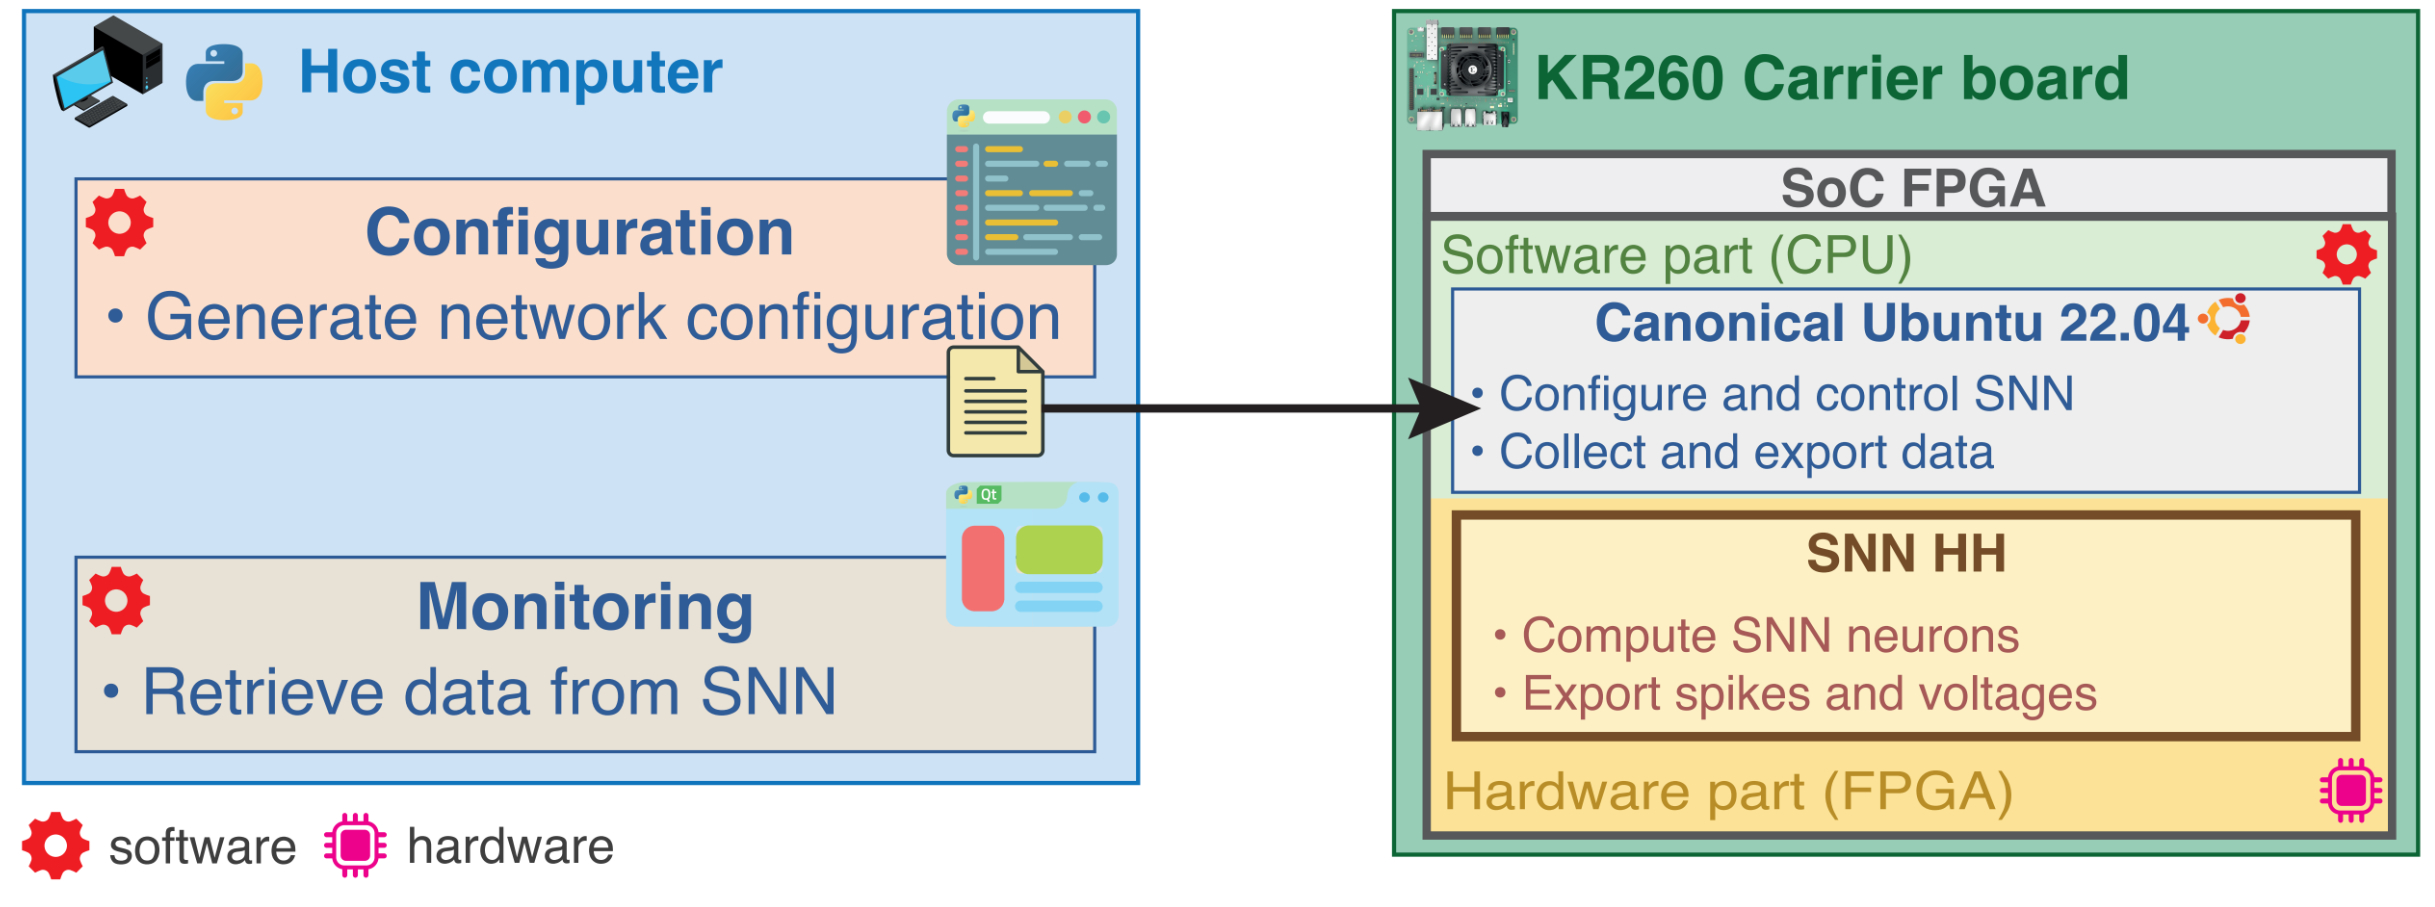
\includegraphics[width=0.9\linewidth]{Figure/Architecture BioEmus.jpg}
    \end{center}
    \caption{Block diagram illustrating the architecture of BioemuS and distinguishing between software and hardware designs through red and pink symbols, respectively.}
    \label{fig:Architecture BioEmus}
\end{figure}

The SNN utilizes Hodgkin-Huxley (HH) neurons \cite{HodgkinHuxley1990}, with preset neuron types including Fast Spiking (FS) and Regular Spiking (RS) neurons (parameters in Table \ref{tab:Neurons and Noise Parameters}; also, refer to Intrinsically Bursting and Low Threshold Spiking neurons, which are not used in this thesis work). Additionally, a biomimetic current simulating synaptic noise, based on the Ornstein-Uhlenbeck process \cite{Destexhe2001} as described by \cite{Khoyratee2019}, is employed to replicate spontaneous activity within the network neurons (parameters in Table \ref{tab:Neurons and Noise Parameters}). 

\begin{table}[!ht]
\centering
\small
\tabcolsep=0.11cm
\begin{tabular}{lccccc}
\hline Parameter & FS & RS & IB & LTS & Unit \\
\hline$g_{N a}$ & 0.05 & 0.05 & 0.05 & 0.05 & $S / \mathrm{cm}^2$ \\
$g_K$ & 0.01 & 0.005 & 0.005 & 0.005 & $S / \mathrm{cm}^2$ \\
$g_M$ & 0.0 & $7 \times 10^{-5}$ & $3 \times 10^{-5}$ & $3 \times 10^{-5}$ & $\mathrm{~S} / \mathrm{cm}^2$ \\
$g_L$ & 0.0 & 0.0 & $1 \times 10^{-4}$ & 0.0 & $\mathrm{~S} / \mathrm{cm}^2$ \\
$g_T$ & 0.0 & 0.0 & 0.0 & $4 \times 10^{-4}$ & $\mathrm{~S} / \mathrm{cm}^2$ \\
$g_{\text {Leak }}$ & 0.00015 & 0.0001 & $1 \times 10^{-5}$ & $1 \times 10^{-5}$ & $\mathrm{~S} / \mathrm{cm}^2$ \\
$E_{N a}$ & 50.0 & 50.0 & 50.0 & 50.0 & $\mathrm{mV}$ \\
$E_K$ & -100.0 & -100.0 & -90.0 & -100.0 & $\mathrm{mV}$ \\
$E_{\text {Ca }}$ & 0.0 & 0.0 & 120.0 & 120.0 & $\mathrm{mV}$ \\
$E_{\text {Leak }}$ & -70.0 & -70.0 & -70.0 & -75.0 & $\mathrm{mV}$ \\
$v_{\text {init }}$ & -70.0 & -70.0 & -70.0 & -75.0 & $\mathrm{mV}$ \\
$\mu_{\text {noise }}$ & 0.048 & 0.042 & 0.042 & 0.042 & 1 \\
$\theta_{\text {noise }}$ & 8.0 & 8.0 & 8.0 & 8.0 & 1 \\
$\sigma_{\text {noise }}$ & 0.11 & 0.09 & 0.09 & 0.09 & 1 \\
$I_{\text {stim }}$ & 0.03 & 0.03 & 0.03 & 0.03 & $\mathrm{~mA} / \mathrm{cm}^2$ \\
area & $\left(67 \times 10^{-4}\right)^2$ & $\left(96 \times 10^{-4}\right)^2$ & $\left(96 \times 10^{-4}\right)^2$ & $\left(96 \times 10^{-4}\right)^2$ & $\mathrm{~cm}^2$ \\
$c_{\text {mem }}$ & 1.0 & 1.0 & 1.0 & 1.0 & $\mu \mathrm{F} / \mathrm{cm}^2$ \\
\hline
\end{tabular}
\caption{Parameters of the HH model and noise for the 4 preset types of neurons tunable from the Python scripts.}
\label{tab:Neurons and Noise Parameters}
\end{table}

Fast and slow excitation and inhibition synapses (AMPAR, NMDAR, GABA\textsubscript{A}R, GABA\textsubscript{B}R) connect neurons in the SNN, with parameters detailed in Table \ref{tab:Synapses Parameters}. 

\begin{table}[!ht]
\centering
\small
\tabcolsep=0.11cm
\begin{tabular}{lccccc}
\hline Parameter & AMPAR & NMDAR & GABA$_{\mathrm{A}} \mathrm{R}$ & GABA$_{\mathrm{B}} \mathrm{R}$ & Unit \\
\hline$g$ & 0.35 & 0.3 & 0.25 & 1.0 & $n S$ \\
$E$ & 0 & 0 & -80 & -95 & $\mathrm{mV}$ \\
$\alpha$ & $1.1 \times 10^6$ & $7.2 \times 10^6$ & $5 \times 10^6$ & - & $\mathrm{M}^{-1} \mathrm{sec}^{-1}$ \\
$\beta$ & 190 & 6.6 & 180 & - & $\mathrm{sec}^{-1}$ \\
$K_1$ & - & - & - & $9 \times 10^4$ & $\mathrm{M}^{-1} \mathrm{sec}^{-1}$ \\
$K_2$ & - & - & - & 1.2 & $\mathrm{sec}^{-1}$ \\
$K_3$ & - & - & - & 180 & $\mathrm{sec}^{-1}$ \\
$K_4$ & - & - & - & 34 & $\mathrm{sec}^{-1}$ \\
$K_d$ & - & - & - & 100 & $\mu M^4$ \\
$n$ & - & - & - & 4 & 1 \\
\hline
\end{tabular}
\caption{Parameters of the 4 types of synapses tunable from the Python scripts.}
\label{tab:Synapses Parameters}
\end{table}

Moreover, the configuration scripts allowed the setup of the ratio between excitatory and inhibitory neurons, the ratio between fast and slow synapses, the synaptic weight, and the connection probability between neurons, according to custom equations. Equation \ref{eq:Synaptic Connection Rule} represents the connection rule used to connect two neurons and illustrates how the connection probability varies linearly based on their distance from each other:

\begin{equation}
p = p_{max} (1-\frac{d_{npre-npost}}{d_{net}})
\label{eq:Synaptic Connection Rule}
\end{equation}

where $p$ is the probability of connection between two neurons, $p_{max}$ is the maximum probability of connection between two neurons, $d_{npre-npost}$ is the distance between the presynaptic and postsynaptic neuron, $d_{net}$ is the diameter of the neuronal network. 

Equation \ref{eq:Synaptic Connection Rule}, together with a custom procedure for the cluster-like positioning of the neurons in the network, favored the creation of a network topology resembling the small-world one, with more connections within the same cluster and less between clusters as depicted in Figure \ref{fig:Network Topology}.

\begin{figure}[ht!]
    \begin{center}
    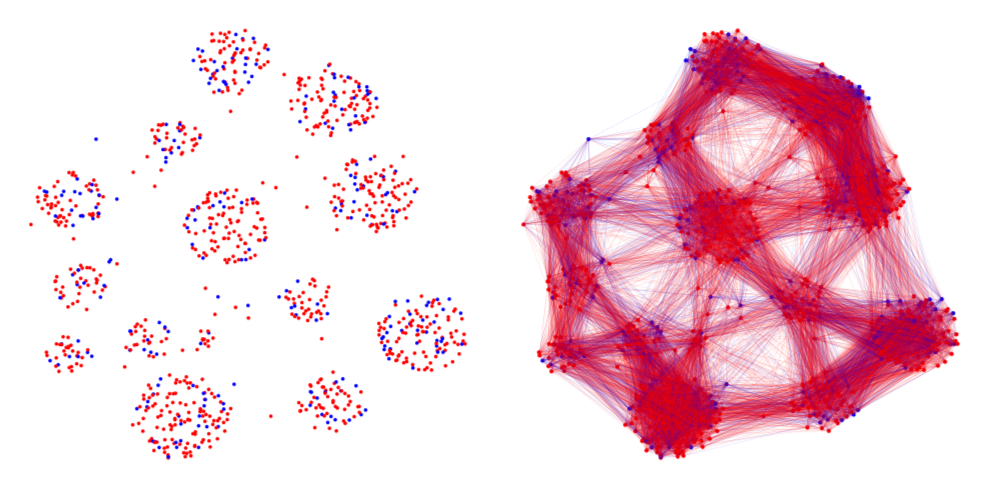
\includegraphics[width=0.9\linewidth]{Figure/Network Topology.jpg}
    \end{center}
    \caption{Position of the neurons (left) and their connections (right) of the simulated network. Blue dots are inhibitory neurons that make inhibitory synapses (blue lines) while red dots are excitatory neurons that make excitatory synapses.}
    \label{fig:Network Topology}
\end{figure}

The time step for the computation of the neuron is 2\textsuperscript{-5} ms, as in \cite{Khoyratee2019}, to ensure satisfactory stability and accuracy in the system solving with Forward Euler solving. Additionally, spikes are compressed over a time stamp of 1 ms, resulting in a spike train with a frequency of 1000 Hz.

In this work, a bank of 325 spiking neural networks, each comprising 1024 neurons, was emulated for 10 minutes each, varying the values of the specified configuration parameters. To maintain consistency in the positions and connections of the network's neurons, a seed was utilized to eliminate variability in the network's topology generation algorithm. This approach ensured a fairer comparison between the networks.

\subsection{Data and Statistical Analyses}

\subsubsection{Data Processing}

All the in-vivo recordings were preprocessed as described in the previous chapter in the section "Preprocessing". The subsequent characterization of the firing activity of both the biological and artificial neural networks was performed using Python. The analyses focused on several biomarkers, including Inter-Spike Interval (ISI, ms), Mean Firing Rate (MFR, spikes/s), Mean Bursting Rate (MBR, bursts/min), Pearson’s Correlation (PC), and Burstiness Index (BI). For these analyses all the detected neurons were considered.

\subsubsection{Mean Firing Rate (MFR)} 

The level of the neuronal firing was evaluated computing the mean firing rate that calculates the average number of spikes in the unit of time (s). 

\subsubsection{Inter-Spike Interval (ISI)}

The inter-spike intervals were analyzed computing the ISI histogram (ISIH) by aggregating the ISIs of all sorted neurons in each network.

\subsubsection{Mean Bursting Rate (MBR)}

The level of the neuronal bursting was evaluated computing the mean bursting rate that calculates the average number of bursts in the unit of time (min). The bursts were detected using the string method (i.e. a max inter-spike interval of 100 ms and 5 as minimum number of intra-burst spikes) according to \cite{Chiappalone2005}.  

\subsubsection{Pearson's Correlation (PC)}

For the computation of the Pearson's coefficient, the method explained in \cite{Selinger2004} was used, with a bin of 200 ms. It's an algorithm that aims to capture the correlation between the neurons of the network.

\subsubsection{Burstiness Index (BI)}

The burstiness index algorithm and its parameters were consistent with those described in \cite{Wagenaar2005}. Its objective is to assess the level of network synchronization without directly analyzing burst activity, thereby circumventing the limitations introduced by burst detection algorithms.

\subsubsection{Statistical Analysis}

The statistical analysis was performed in Python. Only those neurons, either from the SNNs or the six BNNs, with a MFR greater than 0.5 spikes/s were considered for performing the one-way ANOVA test on the log-transformed MFR. P-values were considered significant for $p<0.0001$.

\section{Results}

\subsection{Performances of the simulated SNNs}

A method was devised to identify the most relevant SNN configurations from a range of constructed models. A comparative analysis was carried out between the BNNs, considered as the reference, and the 325 SNNs. This comparison relied on the Root Mean Square deviation (RMSE), calculated between the median inter-spike interval histogram (ISIH) trends of the biological network and the one of each SNN. Additionally, comparisons between the artificial and the biological networks were executed by assessing the differences in the median values of key biomarkers defined in the previous section, i.e. MFR, MBR, PC, and BI. According to this, a grading system was established by computing the absolute value of the distance between each biomarker computed for the SNN and the target value (i.e. the median) of the same biomarker for the BNN. These differences (in absolute values) were then normalized considering the maximum and minimum values of each biomarker among all the configurations, as depicted in the following Equation \ref{eq:Grading Formula}:

\begin{equation}
Grade = 1 - \left[\frac{\left|diff_{i,m}\right|-min(\left|diff_{m}\right|)}{max(\left|diff_{i,m}\right|-min(\left|diff_{m}\right|))}\right] 
\label{eq:Grading Formula}
\end{equation}

where $diff_{i,m}$ is the i-th difference between the m-th biomarker of the i-th SNN configuration and the target value of the same biomarker of the BNN.

By computing all the grades for the several identified biomarkers, the radar plot, depicted in Figure \ref{fig:Radar Plot Grades}, was obtained where the distribution of all the 325 SNN configurations (grey lines) can be appreciated. 

\begin{figure}[ht!]
    \begin{center}
    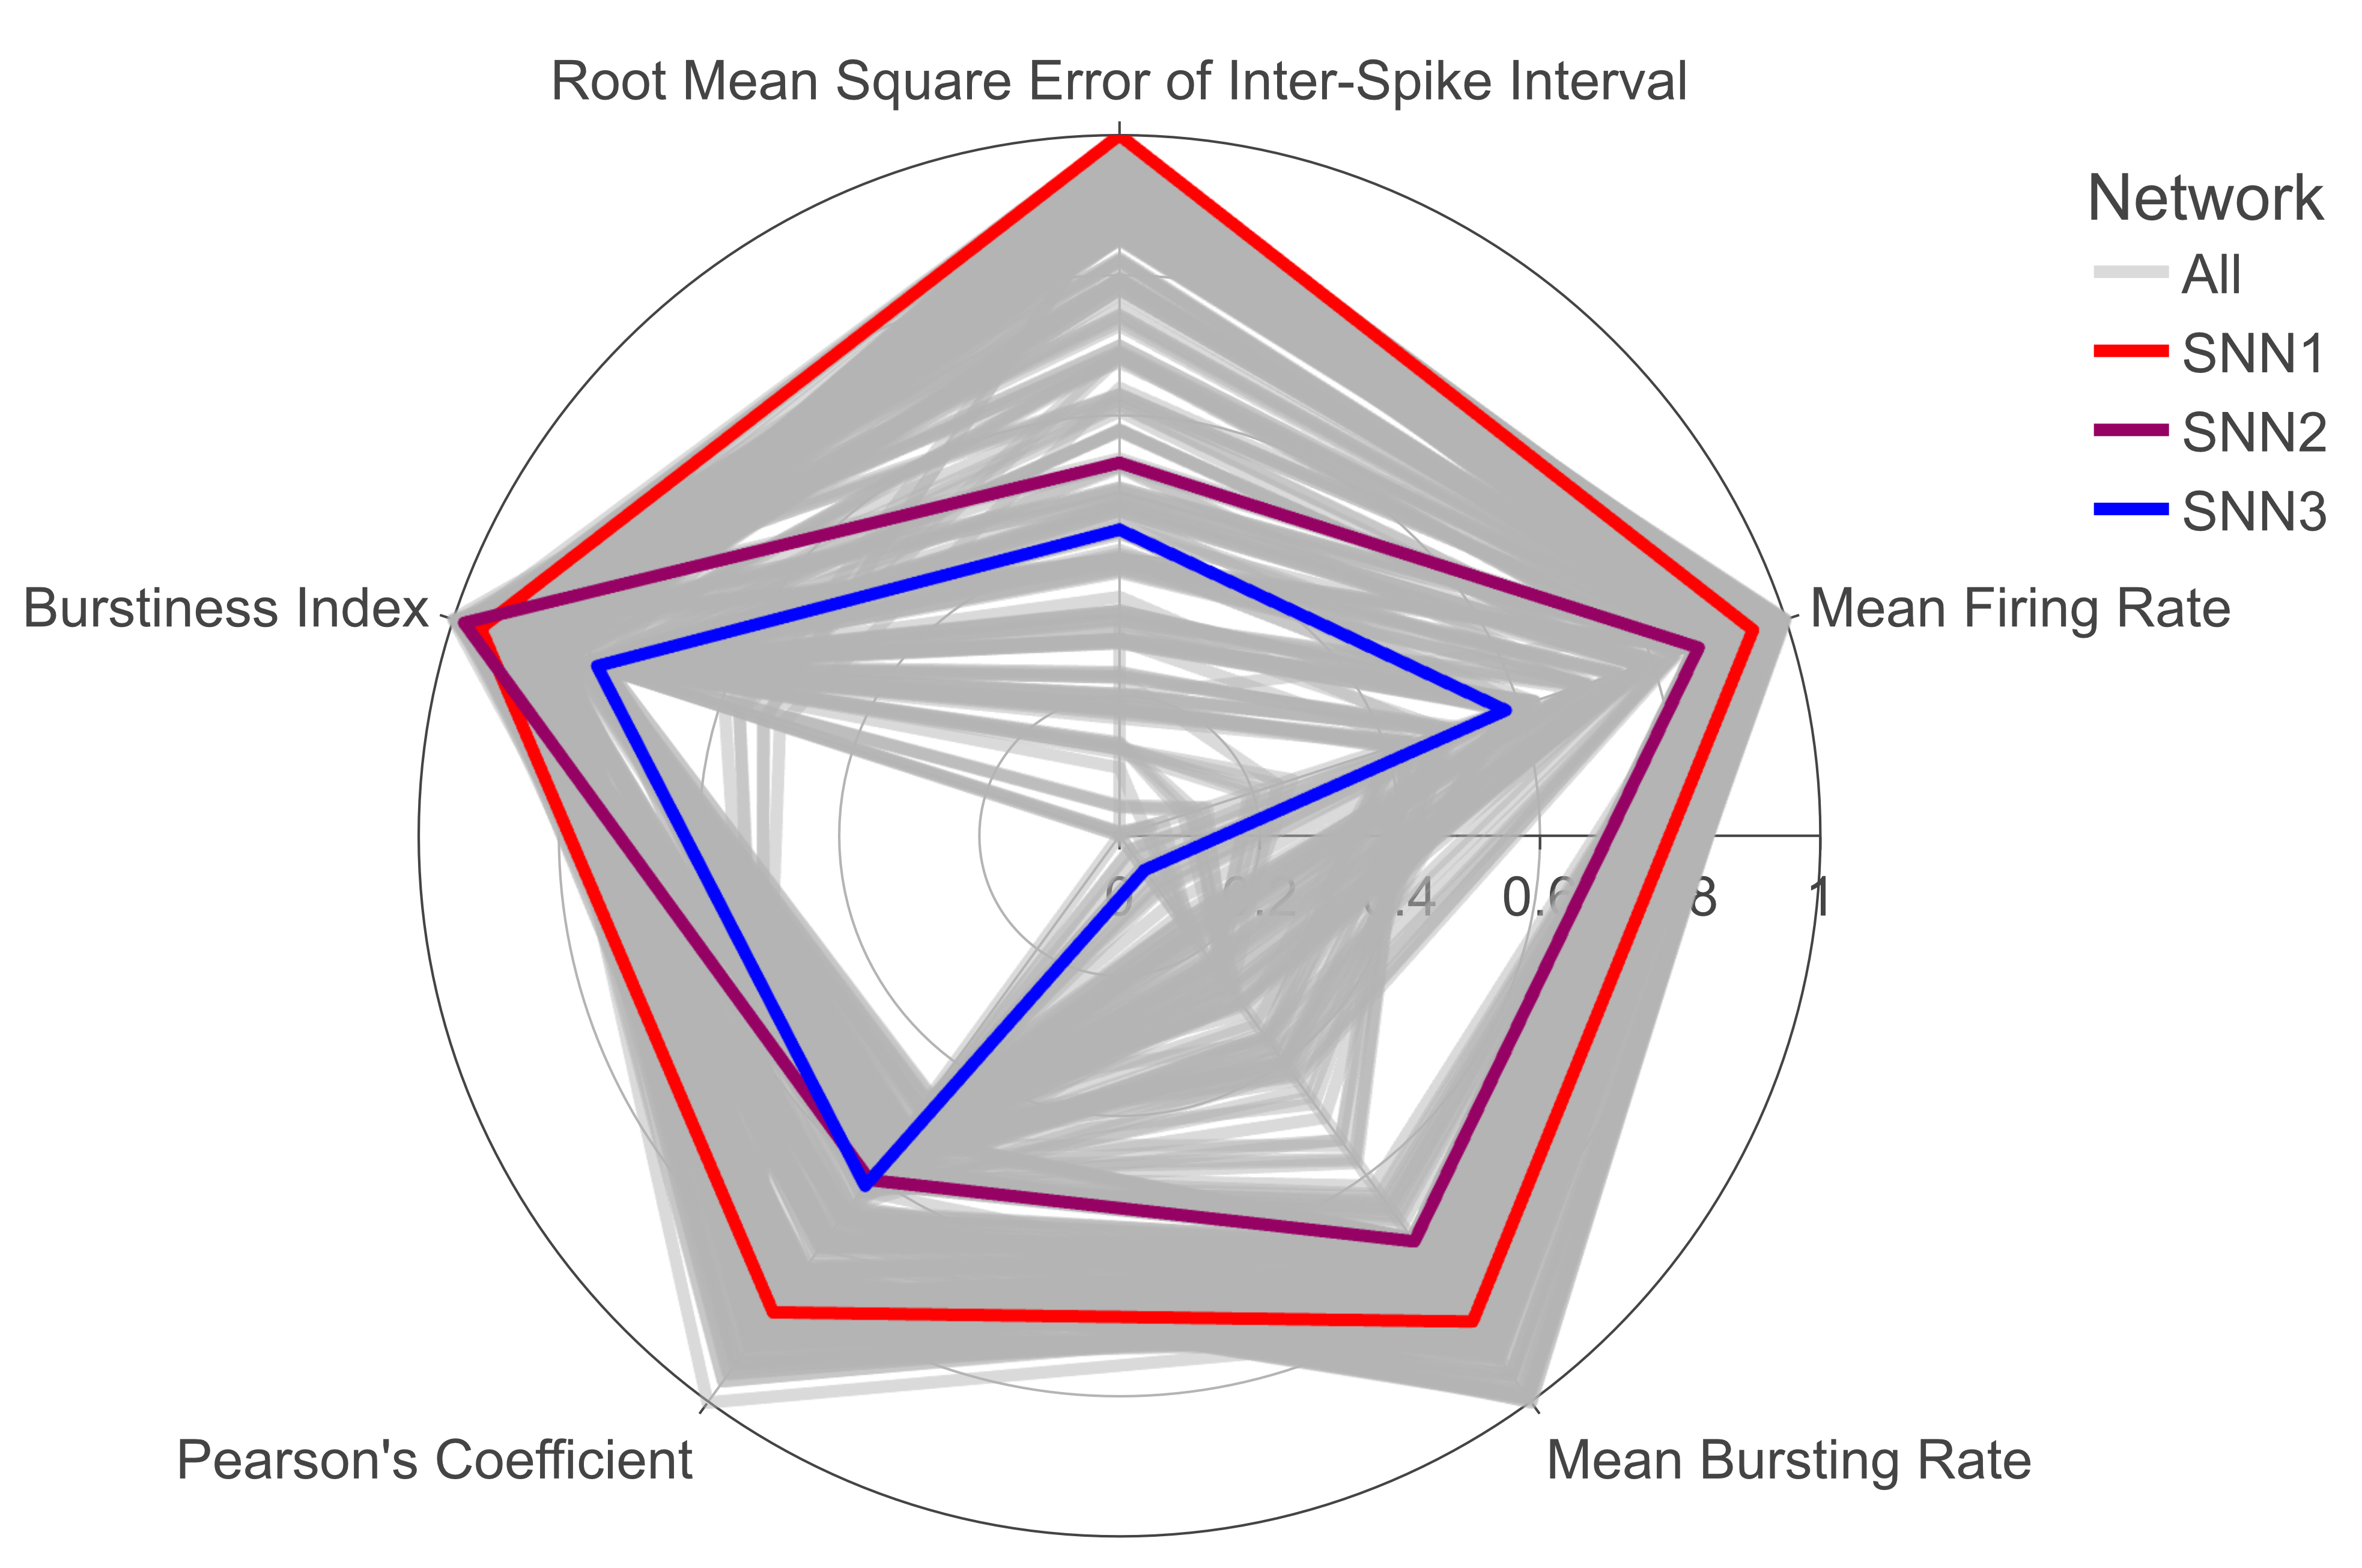
\includegraphics[width=\linewidth]{Figure/Radar Plot Grades.jpg}
    \end{center}
    \caption{Radar plot of the selected network biomarkers, which are: Root Mean Square Error of the Inter Spike Interval (RMSE), Mean Firing Rate (MFR), Mean Bursting Rate (MBR), Pearson’s Coefficient (PC), and Burstiness Index (BI). The plot for each configured SNN is represented in grey. SNN1 is highlighted in red, exhibiting a plot that covers a larger area. SNN2, shown in blue, has a plot covering a median area, while SNN3, depicted in purple, covers one of the smallest areas.}
    \label{fig:Radar Plot Grades}
\end{figure}

Three configurations have been highlighted among all the available: one exemplifying the network with the highest score (SNN1, depicted by the red line), and two additional instances (SNN2 and SNN3, illustrated by the purple and blue lines, respectively) characterized by lower scores, suggesting deviations from the BNN. This choice enabled the assessment of how fine-tuning affects the electrophysiological activity of individual networks.

Ultimately, the overall grade for each specific configuration was established by multiplying each normalized value with respect to various biomarkers, as outlined in Table \ref{tab:Network Performance} for the three selected SNNs. It can be observed that SNN1 obtains the highest score, SNN2 falls in the median range, and SNN3 receives the lowest score among those selected.

\begin{table}[!ht]
\centering
\small
\tabcolsep=0.11cm
\begin{tabular}{|l|c|c|c|c|c|c|}
\hline \multirow{2}{*}{ Network } & \multicolumn{6}{|c|}{ PERFORMANCE VOTE } \\
\cline { 2 - 7 } & MFR & MBR & \begin{tabular}{c} 
RMSE \\
of ISI
\end{tabular} & PC & BI & \begin{tabular}{c} 
FINAL \\
GRADE
\end{tabular} \\
\hline SNN1 & 0.95 & 0.86 & 1 & 0.84 & 0.96 & 0.66 \\
\hline SNN2 & 0.87 & 0.72 & 0.53 & 0.61 & 0.98 & 0.20 \\
\hline SNN3 & 0.58 & 0.6 & 0.44 & 0.62 & 0.78 & 0.01 \\
\hline
\end{tabular}
\caption{Network Performance.}
\label{tab:Network Performance}
\end{table}

\subsection{Comparing artificial and biological neural 
networks}

A comparative study was performed to evaluate the firing dynamics of the selected SNNs and the target BNN. Figure \ref{fig:Histo-Box Comparison SNN-BNN}A reports the ISI histogram profiles of the chosen SNNs (SNN1 in red, SNN2 in purple, SNN3 in blue) and the pool of the six BNNs (in black, with the confidence interval shaded). 

\begin{figure}[ht!]
    \begin{center}
    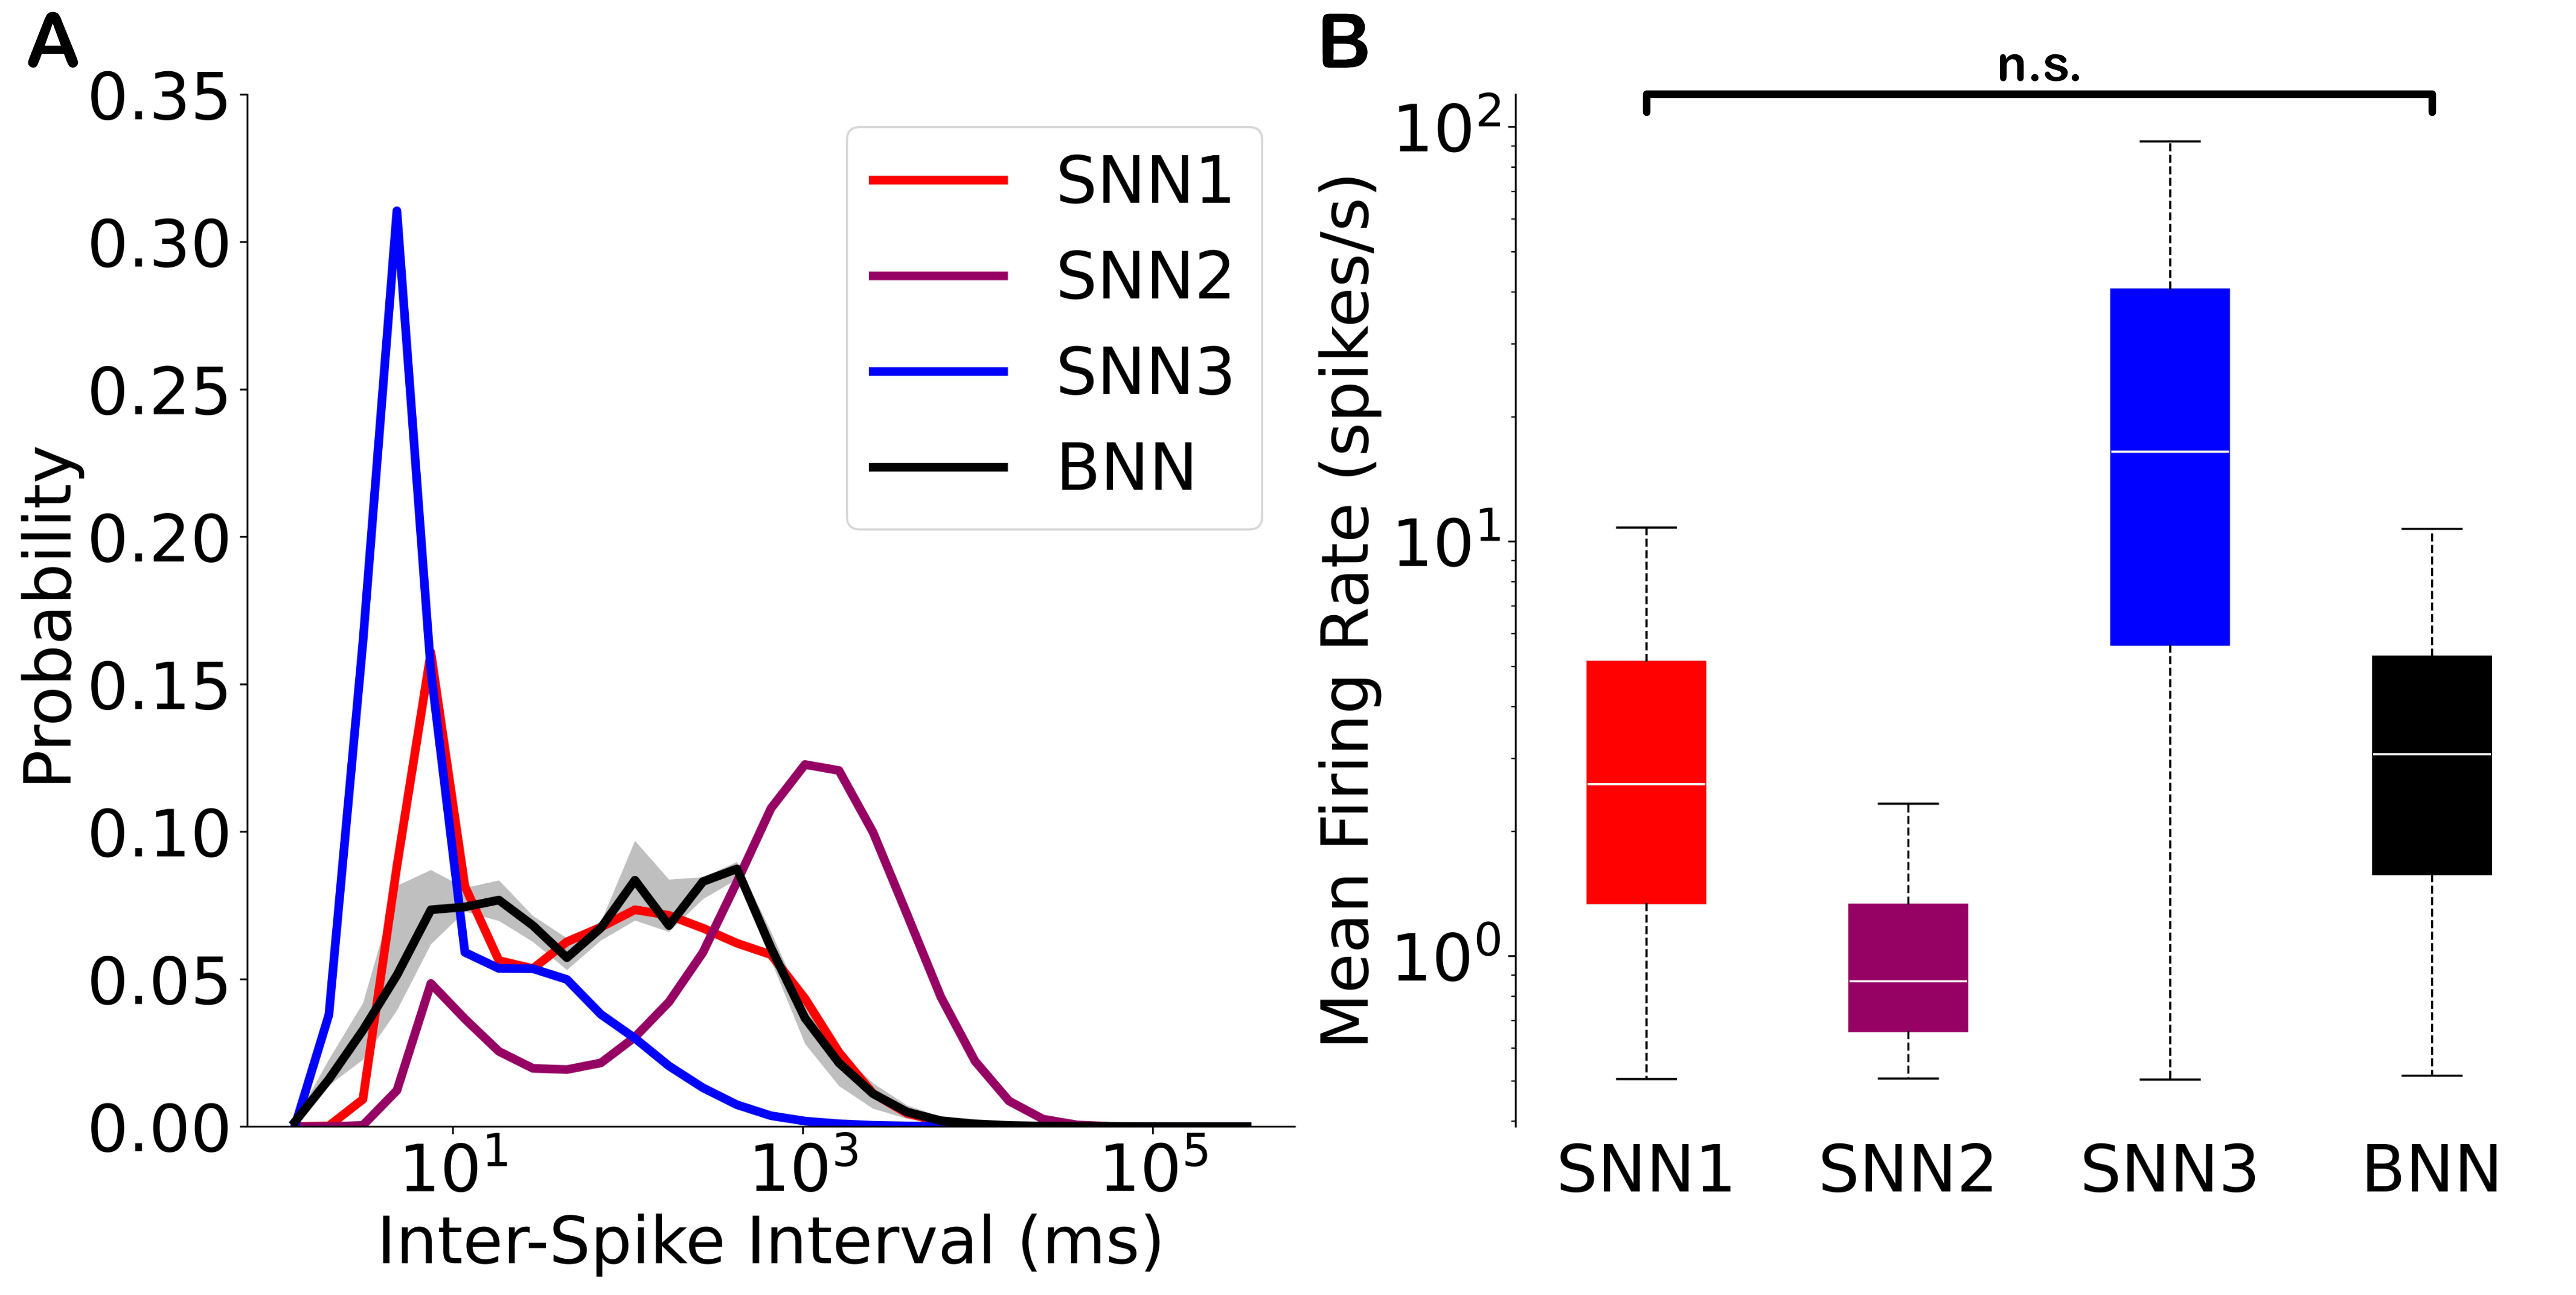
\includegraphics[width=\linewidth]{Figure/Histo-Box Comparison SNN-BNN.jpg}
    \end{center}
    \caption{Comparative analysis between BNNs and SNNs. (A) Inter Spike Interval Histograms (ISIHs) of three SNNs and the median trend of ISIHs from six selected rats. The shaded area denotes the range between the 25th and 75th percentiles. (B) MFR boxplots of all the single units in the three SNNs and the BNN. The BNN data were obtained by pooling together all single-unit activity of 6 rats. The central white line of the boxplots represents the median, while the top and bottom of the boxes are the 25-th and 75-th percentiles. The whiskers show the Q1-1.5*IQR and Q3+1.5*IQR, where Q1 and Q3 are the first and third quartiles, while the IQR is the interquartile range.}
    \label{fig:Histo-Box Comparison SNN-BNN}
\end{figure}

A first, qualitative evaluation indicates a good match between SNN1 and the pool of BNNs, which deviates from the profile of both SNN2 and SNN3. This is in accordance with the scores obtained in Table \ref{tab:Network Performance}, indicating SNN1 as the configuration better resembling the activity of the in vivo biological network. This is also confirmed by statistical analysis performed on the firing rate (Figure \ref{fig:Histo-Box Comparison SNN-BNN}B), for which SNN1 values do not significantly differ from those of the BNNs ($p= 0.477$, one-way ANOVA). For all the other network comparisons, the null hypothesis was rejected ($p<0.0001$, one-way ANOVA Figure \ref{fig:Histo-Box Comparison SNN-BNN}B). 

Furthermore, the raster plots presented in Figure \ref{fig:Raster Comparison SNN-BNN} offer a clear, even if qualitative, representation of the obtained electrophysiological activity for the optimal SNN (i.e. SNN1), the low-scored SNN2 and SNN3 and one representative in vivo network from rat. Indeed, SNN1 is the one better resembling the spike pattern of the BNN.

\begin{figure}[ht!]
    \begin{center}
    \includegraphics[width=\linewidth]{Figure/Raster Comparison SNN-BNN.jpg}
    \end{center}
    \caption{Comparative analysis between BNNs and SNNs. 20-s raster plot showing the firing activity of 30 neurons of each considered network.}
    \label{fig:Raster Comparison SNN-BNN}
\end{figure}

\section{Discussion and Conclusion}

In this study, a real-time Spiking Neural Network (SNN) was introduced to replicate key electrophysiological properties observed in an in vivo neuronal network. A dataset of six experiments on anesthetized rats was utilized to identify the target dynamics of the reference Biological Neural Network (BNN). Using BioemuS, a custom-developed FPGA-based platform containing 1024 single-compartment Hodgkin-Huxley neurons and 2\textsuperscript{20} synapses, simulations were conducted for 325 different SNNs. A procedure was developed to select the optimal SNN configuration capable of emulating the electrophysiological behavior of the BNN. The identified SNN exhibited primary biomarkers typical of in vivo cortical networks, such as firing and bursting rates, correlation levels, burstiness index, and Inter Spike Interval histogram. These results represent an important milestone for the future development of experiments where the SNN will drive the stimulation in vivo, paving the way for innovative neuromorphic-based neuroprostheses \cite{Chiappalone2022}.